\documentclass{article}

\title{Splay Trees}
\date{September 12, 2005}
\author{Lecturer: David Karger\\ Scribes: Xin Zhang, Zeyuan Allen Zhu (revised 2011)}

\begin{document}

%%%%%%%%%%%%%%%%%%%%%%%%%%%%%%%%%%%%%%%%%%%%%%%%%%%%%%%%%%%%%%%%%%%%%

%%%%%%%%%%%%%%%%%%%%%%%%%%%%%%%%%%%%%%%%%%%%%%%%%%%%%%%%%%%%%%%%%%%%%%
% Your notes start here!
%%%%%%%%%%%%%%%%%%%%%%%%%%%%%%%%%%%%%%%%%%%%%%%%%%%%%%%%%%%%%%%%%%%%%%
%
% For theorems, lemmas, definitions, remarks, etc. use commands
% {\theorem{...}}, {\lemma{...}}, {\definition{...}}, etc.
% For proofs, use \begin{proof} ... \end{proof}
%
% For postscript figures (.ps) use the following block:
%
% \begin{figure}[h]
% \begin{center}
% \mbox{\psfig{figure=notes-nn-fig-mm.ps}}
% \caption{A very nice picture.}
% \label{fig:picture}
% \end{center}
% \end{figure}
%

% For encapsulated postscript figures (.eps) use the following block:
%  (also change documentstyle line )
% \begin{figure}[h]
% \begin{center}
% \mbox{\includegraphics[width=0.75\textwidth]{notes-nn-fig-mm.eps}}
% \caption{A very nice picture.}
% \label{fig:picture}
% \end{center}
% \end{figure}
%


%%%%%%%%%%%%%%%%%%%%%%%%%%%%%%%%%%%%%%%%%%%%%%%%%%%%%%%%%%%%%%%%%%%%%%

\section{Introduction}

Splay trees are binary search trees with good balance properties when
amortized over a sequence of operations. It does not require extra marking fields, like the color field in the red-black tree.

When a node $x$ is accessed, we perform a sequence of \textbf{splay steps}
to move $x$ to the root of the tree. There are 6 types of splay steps,
each consisting of 1 or 2 rotations (see Figures \ref{fig:splaystep_rr},
\ref{fig:splaystep_lr}, and \ref{fig:splaystep_r}).

\begin{figure}[ht]
\begin{center}
  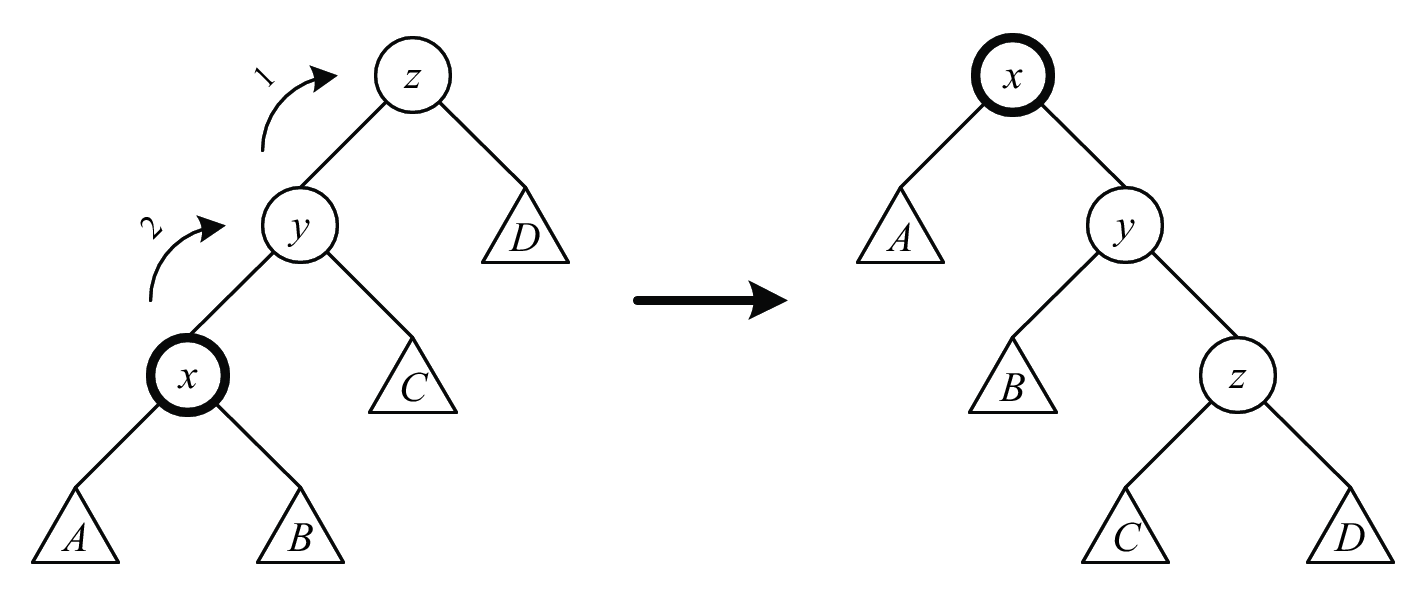
\includegraphics{dzhang-splaystep-rr.png}
  \caption{\textbf{The $rr$ (zig-zig) splay step:} This is performed when $x$ and
$x$'s parent are both left children. The splay step consists of first
a right rotation on $z$ and then a right rotation on $y$ (hence $rr$).
The $ll$ (zag-zag) splay step, for $x$ and $x$'s parent being right children, is
analogous.}
\label{fig:splaystep_rr}
\end{center}
\end{figure}

\begin{figure}[ht]
\begin{center}
  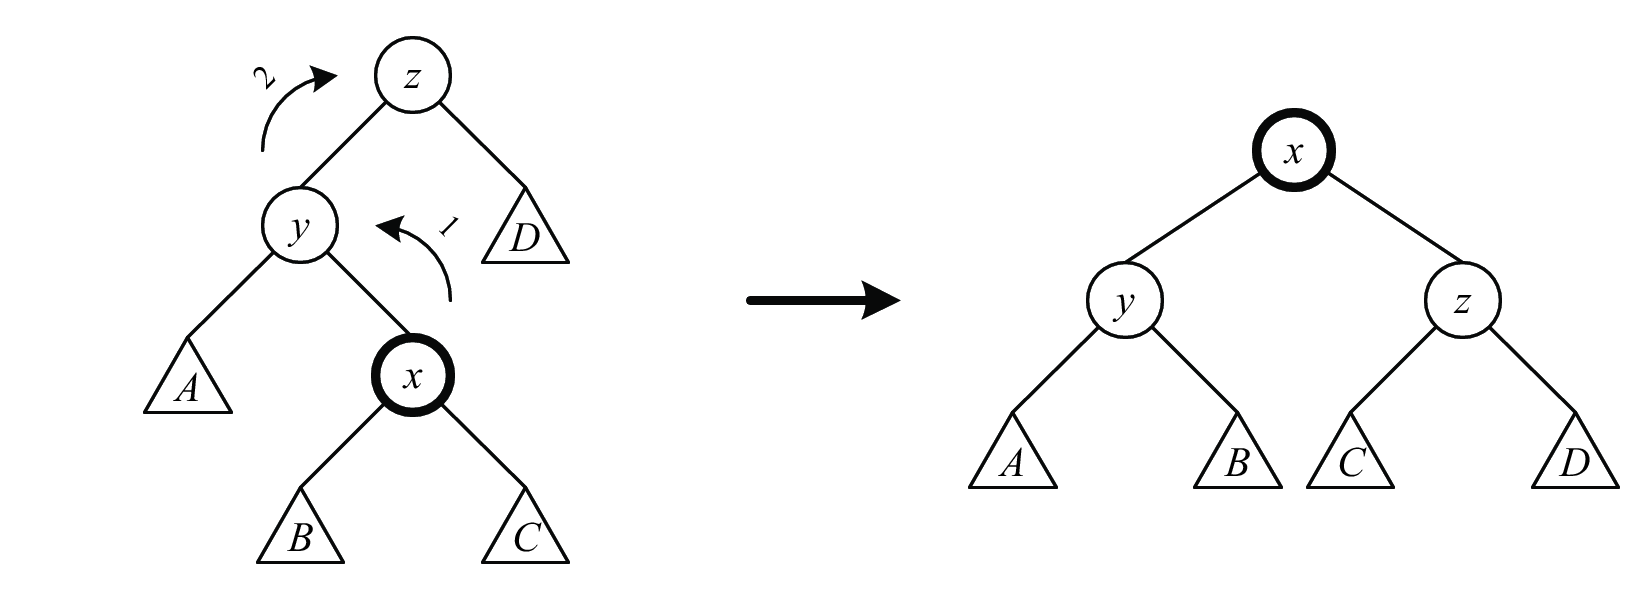
\includegraphics{dzhang-splaystep-lr.png}
\caption{\textbf{The $lr$ (zig-zag) splay step:} This is performed when $x$ is
a right child and $x$'s parent is a left child. The splay step consists
of first a left rotation on $y$ and then a right rotation on $z$.
The $rl$ (zag-zig) splay step, for $x$ being a left child and $x$'s parent being
a right child, is analogous.}
\label{fig:splaystep_lr}
\end{center}
\end{figure}

\begin{figure}[ht]
\begin{center}
  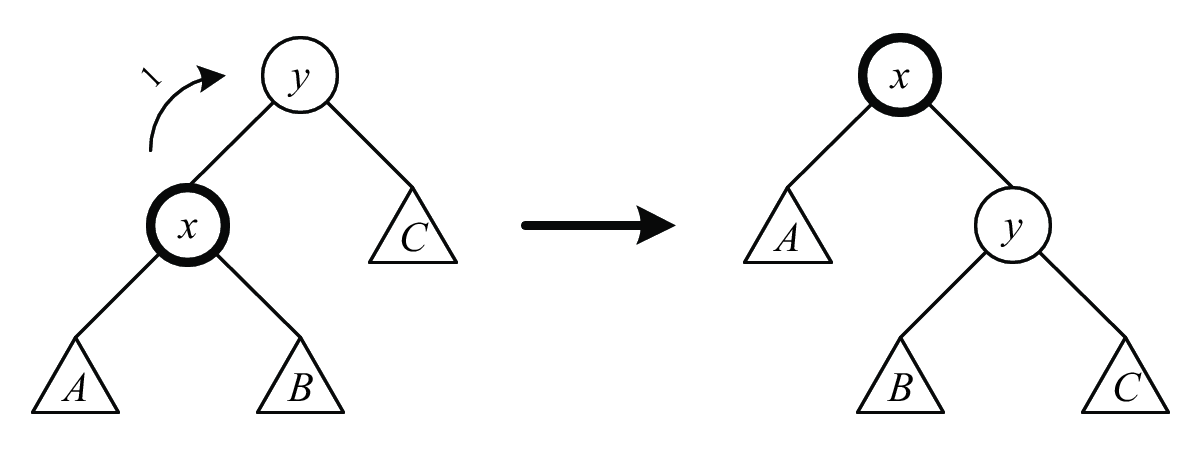
\includegraphics{dzhang-splaystep-r.png}
\caption{\textbf{The $r$ (zig) splay step:} This is performed when $x$ is
the left child of the root $y$. The splay step consists of a right
rotation on the root. The $l$ splay step, for $x$ being the right
child of the root, is analogous.}
\label{fig:splaystep_r}
\end{center}
\end{figure}

We perform splay steps to $x$ ($rr$, $ll$, $lr$, or $rl$, depending on
whether $x$ and $x$'s parent are left or right children) until $x$
is either the root or a child of the root. In the latter case, we need
to perform either a $r$ or $l$ splay step to make $x$ the root.
This completes a \textbf{splay} of $x$.

One intuition behind this is that the most recently used node is now moved to the root, and therefore this will speed up further queries to this node. Another, and arguably more important intuition is that, it also helps further queries to other nodes, because a splay operation will move up the nodes that are deep in the tree, as we will see in the next subsection.
In general, the cost of performing this operation will be absorbed by the potential of a node, which measures the 'fatness' of a node.

We will show that splay operations have amortized cost $O(\log n)$,
and that consequently all splay tree operations have amortized cost
$O(\log n)$.

\section{Analysis of Splay Steps}

For amortized analysis, we define the following for each node $x$:
\begin{itemize}
\item a constant \emph{weight} $w(x) > 0$ (for the analysis, this
  can be arbitrary)
\item \emph{weight sum} $s(x) = \sum_{y \in \textrm{subtree}(x)} w(y)$
  (where $\textrm{subtree}(x)$ is the subtree rooted at $x$,
  including $x$)
\item \emph{rank} $r(x) = \log s(x)$
\end{itemize}

We use $r(x)$ as the potential of a node. The potential function
after $i$ operations is thus
$\phi(i) = \sum_{x \in \textrm{tree}} r(x)$.

\textbf{Lemma}:
The amortized cost of a splay step on node $x$ is
$\le 3(r'(x) - r(x)) + 1$, where $r$ is rank before the
splay step and $r'$ is rank after the splay step. Furthermore,
the amortized cost of the $rr$, $ll$, $lr$, and $rl$ splay steps
is $\le 3(r'(x) - r(x))$.

\begin{proof}

We will consider only the $rr$ splay step (refer to
Figure \ref{fig:splaystep_rr}). The actual cost of the
splay step is 2 (for 2 rotations). The splay step only affects
the potentials/ranks of nodes $x$, $y$, and $z$; we observe that
$r'(x) = r(z)$, $r(y) \ge r(x)$, and $r'(y) \le r'(x)$.

The amortized cost of the splay step is thus:
\begin{align*}
  \textrm{amortized cost} & = 2 + \phi(i + 1) - \phi(i) \\
  & = 2 + (r'(x) + r'(y) + r'(z)) - (r(x) + r(y) - r(z)) \\
  & = 2 + (r'(x) - r(z)) + r'(y) + r'(z) - r(x) - r(y) \\
  & \le 2 + 0 + r'(x) + r'(z) - r(x) - r(x) \\
  & = 2 + r'(x) + r'(z) - 2r(x)
\end{align*}

The log function is concave, i.e., $\frac{\log a + \log b}{2} \le
\log\left(\frac{a + b}{2}\right)$. Thus we also have ($s$ is
weight sum before the splay step and $s'$ is weight sum after the
splay step):
\begin{align*}
  \frac{\log(s(x)) + \log(s'(z))}{2} & \le
    \log\left(\frac{s(x) + s'(z)}{2}\right) \\
  \frac{r(x) + r'(z)}{2} & \le
    \log\left(\frac{s(x) + s'(z)}{2}\right)
    \textrm{(note that $s(x) + s'(z) \le s'(x)$)}\\
  & \le \log\left(\frac{s'(x)}{2}\right) \\
  & = r'(x) - 1 \\
  r'(z) & \le 2r'(x) - r(x) - 2
\end{align*}

Thus the amortized cost of the $rr$ splay step is
$\le 3(r'(x) - r(x))$.

The same inequality must hold for the $ll$ splay step; the inequality
also holds for the $lr$ (and $rl$) splay steps. The $+ 1$
in the lemma applies for the $r$ and $l$ cases.

\end{proof}

\textbf{Corollary}:
The amortized cost of a splay operation on node $x$ is $O(\log n)$.

\begin{proof}

The amortized cost of a splay operation on $x$ is the sum of the
amortized costs of the splay steps on $x$ involved:
\begin{align*}
  \textrm{amortized cost} & = \sum_{i}
    \textrm{cost}(\textrm{splay\_step}_{i}) \\
  & \le \sum_{i} \left(3r^{i + 1}(x) - r^{i}(x)\right) + 1 \\
  & = 3(r(\textrm{root}) - r(x)) + 1
\end{align*}

The $+ 1$ comes from the last $r$ or $l$ splay step (if necessary).
If we set $w(x) = 1$ for all nodes in the tree, then
$r(\textrm{root}) = \log n$ and we have:
$$\textrm{amortized cost} \le 3\log n + 1 = O(\log n)$$
\end{proof}

There are more applications mentioned in class, about how to more cleverly set the initial weight $w_i$'s. Please refer to the raw notes.

\section{Analysis of Splay Tree Operations}

\subsection{Find}
For the find operation, we perform a normal BST find followed by a
splay operation on the node found (or the leaf node last encountered,
if the key was not found). We can charge the cost of going down the
tree to the splay operation. Thus the amortized cost of find is
$O(\log n)$.

\subsection{Insert}
For the insert operation, we perform a normal BST insert followed by
a splay operation on the node inserted. Assume node $x$ is inserted at
depth $k$. Denote the parent of $x$ as $y_{1}$, $y_{1}$'s parent as
$y_{2}$, and so on (the root of the tree is $y_{k}$). Then the change
in potential due to the insertion of $x$ is ($r$ is rank before the
insertion and $r'$ is rank after the insertion, $s$ is weight sum
before the insertion):
\begin{align*}
  \Delta\phi & = \sum_{j = 1}^{k} \left(r'(y_{j}) -
    r(y_{j})\right) \\
  & = \sum_{j = 1}^{k} \left(\log(s(y_{j}) + 1) -
    \log(s(y_{j})\right) \\
  & = \sum_{j = 1}^{k}
    \log\left(\frac{s(y_{j}) + 1}{s(y_{j})}\right) \\
  & = \log\left(\prod_{j = 1}^{k}
    \frac{s(y_{j}) + 1}{s(y_{j})}\right)
    \textrm{(note that $s(y_{j}) + 1 \le s(y_{j + 1})$)} \\
  & \le \log\left(\frac{s(y_{2})}{s(y_{1})} \cdot
    \frac{s(y_{3})}{s(y_{2})} \cdots
    \frac{s(y_{k})}{s(y_{k - 1})} \cdot
    \frac{s(y_{k}) + 1}{s(y_{k})}\right) \\
  & = \log\left(\frac{s(y_{k}) + 1}{s(y_{1})}\right) \\
  & \le \log n
\end{align*}

The amortized cost of the splay operation is also $O(\log n)$, and
thus the amortized cost of insert is $O(\log n)$.

We have proved the following:

\textbf{Theorem}:
All splay tree operations have amortized cost $O(\log n)$.

\end{document}
